
\chapter{Estado del Arte}

    \noindent En esta sección nuestro objetivo será realizar una investigación por la literatura y los artículos publicados relacionados con el reconocimiento automático de landmarks cefalométricos en tareas de antropología forense para finalmente justificar nuestra elección en el presente trabajo para tratar de resolver el problema. Para ello utilizaremos la base de datos \textit{Scopus} para realizar la búsqueda y consulta de artículos científico publicados.

    \section{Localización de landmarks cefalométricos en imágenes}

        \noindent Para hacernos una primera idea del estado actual del problema de reconocimiento de landmarks faciales en imágenes realizamos una primera consulta en \textit{SCOPUS} con la siguiente \textit{keyword} restringiendo los artículos a aquellos relacionados con la informática:
        
        \begin{verbatim}
        TITLE-ABS-KEY (facial AND (landmarks OR keypoints)AND  detection ) AND 
        (LIMIT-TO(SUBJAREA , "COMP"))
        \end{verbatim}

        \medskip

        \noindent Tras esto realizamos una segunda búsqueda mucho más concreta al tipo de problema que tratamos de resolver. Usando la siguiente \textit{keyword}:

        \begin{verbatim}
            TITLE-ABS-KEY ((( anthropology  OR  ( anthropology  AND  forensic ) ) AND  
            ( cephalometric  AND  ( landmarks  OR  keypoints ))) OR ((anthropology OR  
            ( anthropology AND forensic)) AND (facial AND (landmarks OR keypoints))))  
            AND (LIMIT-TO(SUBJAREA,"COMP"))
        \end{verbatim}

        \begin{figure}[htpb]
            \centering
            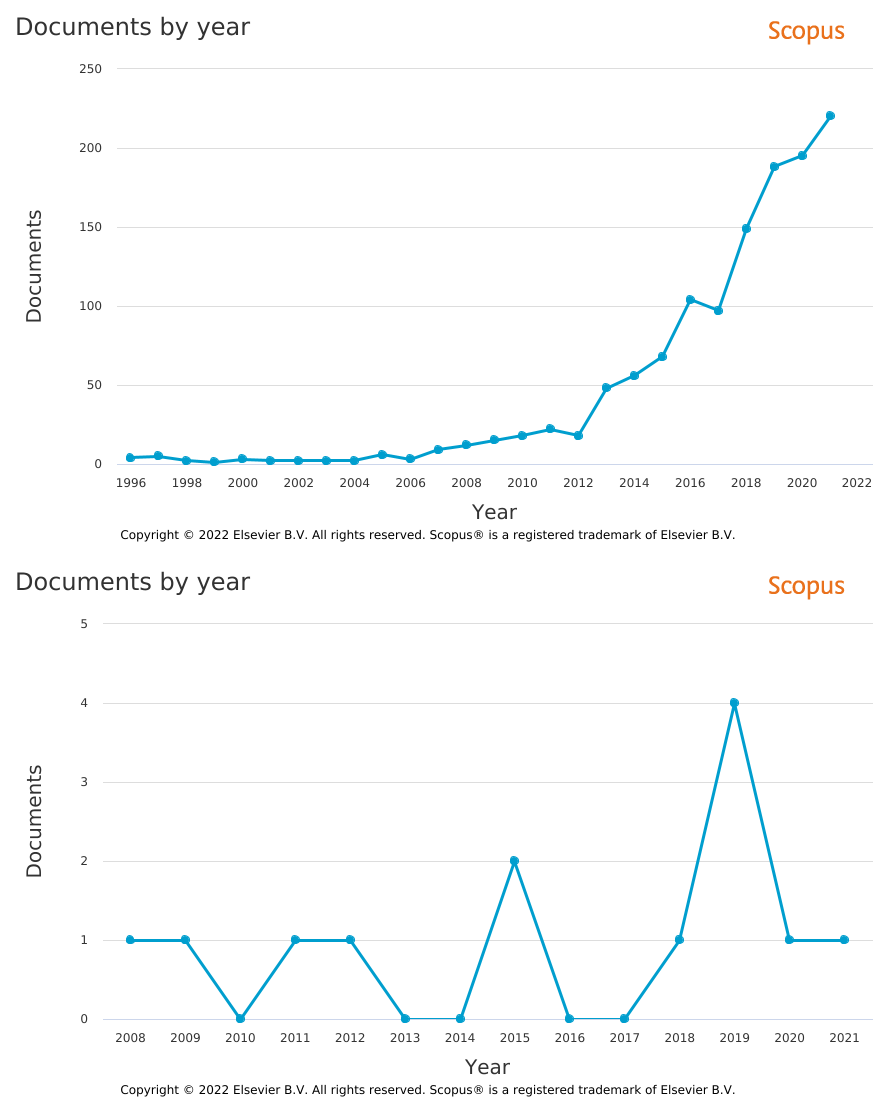
\includegraphics[width=0.9\textwidth]{img/SCOPUS_UNIDOS.png}
            \caption{Arriba podemos ver la gráfica de publicaciones por año obtenida con la primera \textit{keyword} el $26$ de Octubre de $2022$, en total se encontraron $1,251$ artículos. Destaca el notable incremento de papers a partir de 2012, año en que aparece la red AlexNet y comienza a ganar popularidad el Deep Learning en el tratamiento de imágenes. Abajo tenemos la gráfica de publicaciones por año obtenida con la segunda \textit{keyword} el $26$ de Octubre de $2022$, en total se obtuvieron $13$ artículos. Como vemos, existe una gran diferencia entre ambas a nivel de artículos publicados por año.}
            \label{fig:SCOPUS}
        \end{figure}
        
        \medskip
        
        \noindent Como podemos observar en las gráficas generadas para ambas \textit{keywords} en la \autoref{fig:SCOPUS}, actualmente existe una tendencia creciente en la publicación de papers relacionados con este tema, en particular esta tendencia comienza en los años en que surge el Deep Learning y las CNN comienzan a utilizarse en visión por computador para el tratamiento de imágenes. Sin embargo los artículos que se han encontrado no guardan una relación muy estrecha con el problema de deteción de landmarks cefalométricos en problemas de antropología forense. Con la segunda búsqueda anterior se obtienen un total de $14$ artículos, algo que nos confirma que es un área de investigación en la que apenas hay bibliografía o artículos.

        

        \subsection{Evolución en la identificación forense de landmarks cefalométricos}
            
            \noindent Como hemos visto antes, la literatura existente es prácticamente nula, además de los catorce artículos obtenidos con la búsqueda anterior, la mayoría no se centran en el reconocimiento de landmarks cefalométricos en imágenes de rostros, hay artículos que se centran en la superposición craneofacial y otros basados en la identificación de landmarks en cráneos. Por lo tanto, de los catorce artículos vamos a destacar los siguientes por la relación directa con nuestro problema ordenados de mayor a menor antigüedad. Podemos ver una taxonomía en la \autoref{table:taxonomy}. 

            \begin{table}[!ht]
                \centering
                \caption{Taxonomía de los artículos publicados que componen el estado del arte en el campo actualmente.}
                \begin{tabular}{|l|l|l|c|c|c|l|}
                \hline
                    \cellcolor{gray!50}\textbf{Autores} & \cellcolor{gray!50}\textbf{Año} & \cellcolor{gray!50}\textbf{Citas} & \cellcolor{gray!50}\textbf{Bancos de filtros} & \cellcolor{gray!50}\textbf{Aprendizaje Supervisado} & \cellcolor{gray!50}\textbf{CNN} & \cellcolor{gray!50}\textbf{Landmarks}\\ \hline
                    Mohd et al & 2014 & 4 & \cellcolor{gray!15} \textbf{X} & ~ & ~ & 4 \\ \hline
                    Galvánek et al & 2015 & 18 & ~ & ~ & ~ & 14 \\ \hline
                    Faria et al & 2019 & 12 & \cellcolor{gray!15}\textbf{X} & \cellcolor{gray!15}\textbf{X}& \cellcolor{gray!15}\textbf{X} & 28 \\ \hline
                    Anh Tuan et al & 2022 & 1 & ~ & \cellcolor{gray!15}\textbf{X} & \cellcolor{gray!15}\textbf{X}& 16 \\ \hline
                \end{tabular}
                \label{table:taxonomy}
            \end{table}

            \subsubsection{Automatic craniofacial anthropometry landmarks detection and measurements for the orbital region}
                \noindent Se trata de un artículo publicado en $2014$ por Salina Mohd et al \cite{asi2014automatic} en el que se pretende diseñar un método para calcular en una imagen de los ojos de un sujeto el \textit{endocathion} y el \textit{exocanthion} basado en el uso de un clasificador entrenado sobre filtros de Haar usados para la identificación de caras por Viola-Jones.

                \medskip

                \noindent Lo primero que llama la atención del artículo es que tan solo pretende ser capaz de identificar dos landmarks, mientras que en nuestro problema por ejemplo tratamos de predecir la posición de unos treinta (incluyendo en \textit{endocathion} y el \textit{exocanthion}).

                \medskip

                \noindent En segundo lugar, cabe destacar la manera en que se resuelve el problema, pues se hace uso de un clasificador en cascada basado en filtros de tipo Haar. Este es un método tradicional de la visión por computador en el que mediante el paso y convolución de este tipo de filtros por la imagen se obtiene información de esta relativa a los contornos. No obstante se trata de un método que ya se ha visto superado por otras técnicas más recientes de deep learning.

                \medskip

                \noindent Por otro lado, el conjunto de datos que se emplea se ha obtenido en entornos controlados con buena iluminación, algo que no guarda relación con nuestro problema pues se trata de imágenes en diversas posturas, iluminación, y resolución.

            \subsubsection{Automated facial landmark detection, comparison and visualization}
                \noindent Se trata de un trabajo realizado en $2015$ por Marek Galvánek et al. \cite{galvanek2015automated} para la detección automática de landmarks en modelos $3D$ de imágenes de personas. 

                \medskip

                \noindent Los landmarks detectados por el modelo son en total $14$ y todos ellos pertenecen también al conjunto de landmarks que se detectan en este trabajo fin de grado.

                \medskip

                \noindent El algoritmo propuesto se basa en la curvatura de la superficie del modelo $3$D y en la simetría del perfil. En primer lugar se alinea el modelo $3$D con el plano horizontal de Frankfort \autoref{fig:Frankfort}, un plano utilizado por los antropólogos forenses para marcar landmarks. En segundo lugar se realiza un estudio de la curvatura del modelo $3$D en la zona de la nariz, boca y ojos. Finalmente con el perfil del modelo y la simetría se rectifican y perfeccionan los landmarks marcados en etapas previas.

                \begin{figure}[!h]
                    \centering
                    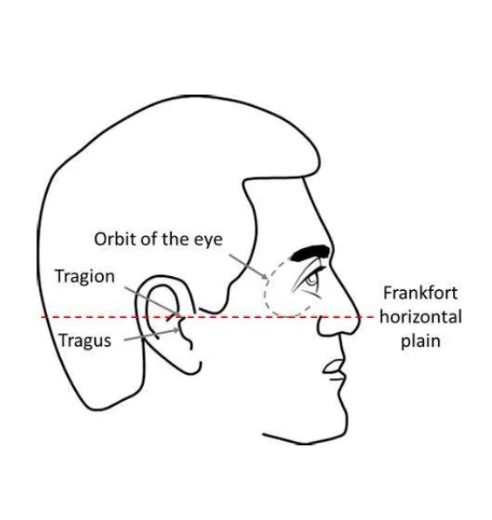
\includegraphics[width=0.5\textwidth]{img/frankfort.png}
                    \caption{Cara alineada con el plano horizontal de Frankfort. Imagen extraida de \url{https://www.slideshare.net/NiharikaSupriya/cephalometrics-landmarkslines-and-planes-93890774
                    }}
                    \label{fig:Frankfort}
                \end{figure}

                \medskip

                \noindent El algoritmo propuesto resulta interesante, aunque no detecta un elevado número de landmarks y se hace de una forma parecida a como un antropólogo forense actuaría. Podemos ver también que es muy preciso en la detección si comparamos los landmarks marcados por el algoritmo con los marcados por un experto manualmente en la \autoref{fig:landmarks_comparativa}.


                \begin{figure}[!h]
                    \centering
                    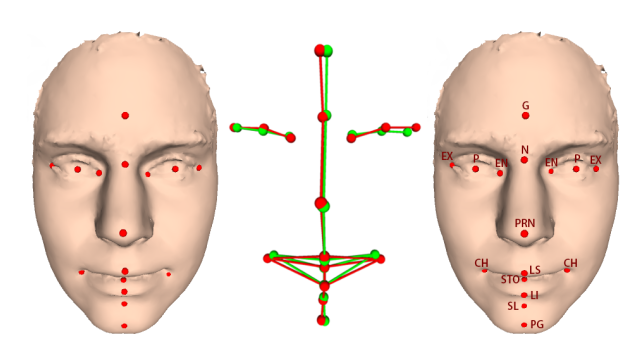
\includegraphics[width=0.8\textwidth]{img/comparativa_landmarks.png}
                    \caption{Comparativa entre los landmarks marcados por el algoritmo desarrollado en el artículo (izquierda) y los marcados por un experto (derecha). Imagen extraida de \cite{galvanek2015automated}.}
                    \label{fig:landmarks_comparativa}
                \end{figure}

                \medskip

                \noindent En este trabajo, comenzamos a ver ya un problema similar al nuestro, la detección automática de landmarks cefalométricos con un mayor número de landmarks ($14$ frente a los $2$ del estudio anterior). Aunque se realiza sobte modelos $3$D de caras que evitan problemas de oclusión, mala iluminación o resolución.

            \subsubsection{Automatic cephalometric landmarks detection on frontal faces: An approach based on supervised learning techniques}

                \noindent El siguiente artículo es de $2019$ y fue realizado por Lucas Faria et al. Pretende desarrollar un algoritmo para el reconocimiento automático de landmarks cefalométricos en imágenes frontales a partir de técnicas de visión por computador y de métodos de aprendizaje supervisado \cite{porto2019automatic}.

                \medskip

                \noindent El algoritmo tiene tres componentes:

                \begin{itemize}
                    \item En la primera fase se realiza un pre-procesamiento de las imágenes para resaltar sus caracteristicas faciales. 
                    \item En la segunda fase se aplica la cascada de filtros de Haar de Viola-Jones para identificar las regiones de interés de la imagen: ojos, nariz, boca.
                    \item Finalmente se aplica el algoritmo de machine learning supervisado a cada una de las regiones anteriores. Creando un detector automático de landmarks para cada región.
                \end{itemize}

                \medskip

                \noindent Por otro lado el conjunto de entrenamiento es de $1000$ individuos de los cuales se tomaron fotografías frontales en las mismas condiciones de iluminación y de distancia a la cámara, por lo que no presenta las mismas complicaciones que el dataset del que disponemos. 

                \medskip

                \noindent Destaca este artículo por ser el primero en el cual comienzan a usarse técnicas de aprendizaje automático para la resolución del problema. Además en las imágenes de entrenamiento fueron marcados 28 landmarks que se emplearon para el entrenamiento, que coinciden con los mismos que tenemos en nuestro problema.

            \subsubsection{The Improved Faster R-CNN for Detecting Small Facial Landmarks on Vietnamese Human Face Based on Clinical Diagnosis}
            
                \noindent Este artículo es el más reciente pues fue publicado en Junio de $2022$ por Ho Nguyen Anh Tuan et al \cite{ImprovedfasterRCNN}. En él se utiliza una versión mejorada de la red faster R-CNN aplicada a la tarea del reconocimiento de landmarks cefalométricos. 

                \medskip

                \noindent Los resultados obtenidos son muy buenos pero como ocurre en la mayoría de trabajos de este tipo, la base de datos usada ha sido de imágenes tomadas de voluntarios en unas mismas condiciones de iluminación frontales y de perfil. 

                \medskip

                \noindent No obstante el trabajo restalta la gran importancia que está teniendo el Deep Learning y las CNN en tareas de reconocimiento de landmarks faciales (usualmente landmarks no biológicos como los que se emplean en tareas de antropología forense), y partiendo de esta base podemos justificar el trabajo que vamos a desarrollar, pues nos proponemos adaptar una red que ya ha sido entrenada para la identificación de landmarks faciales en grandes volúmenes de datos de imágenes en diversas posturas y resolución para la tarea del reconocimiento de landmarks forense.

                \medskip

                \noindent Todos los métodos que se han presentado en esta sección trataban de cumplir con el mismo objetivo, y han ido evolucionando con el paso de los años a la par que la informática, empezando por tratar de aplicar algoritmos coevolutivos, después filtros de Haar y técnicas de visión por computador y finalmente usar CNN de Deep Learning. De esta manera y viendo con perspectiva el estado del arte en el campo, consideramos que la propuesta que presentamos puede traer buenos resultados, pues pretendemos enseñar a un sistema experto en el reconocimiento de landmarks no biológicos a identificar estos otros puntos, lo cual puede suponer un nexo de unión entre las dos líneas de investigación.
   
\endinput
%------------------------------------------------------------------------------------
% FIN DEL CAPÍTULO. 
%------------------------------------------------------------------------------------

